\documentclass[letterpaper,journal]{IEEEtran}
\usepackage{amsmath,amssymb,amsfonts}
\usepackage{array,booktabs,tabularx}
\usepackage{graphicx,xcolor}
\usepackage{algorithm,algorithmic}
\usepackage{tikz}
\usetikzlibrary{arrows.meta,positioning,fit}
\usepackage{pgfplots}
\pgfplotsset{compat=1.18}
\usepackage{cite,url}
\usepackage[hidelinks]{hyperref}
\hypersetup{pdftitle={FreqDuet: Frequency-Informed Coordination of Dynamic Bus Timetables and Holding Budgets},pdfauthor={Anonymous Authors}}
\newcommand{\E}{\mathbb{E}}
\newcommand{\clip}{\operatorname{clip}}
\newcommand{\pos}[1]{[#1]_+}
\newcolumntype{Y}{>{\raggedright\arraybackslash}X}
\hyphenation{time-table time-tables co-or-di-na-tion}
\begin{document}
\title{FreqDuet: Frequency-Informed Coordination of Dynamic Bus Timetables and Holding Budgets}
\author{Anonymous Authors}
\markboth{DEVELOPMENT STUDY --- MANUSCRIPT DRAFT, NOVEMBER 2026}{Frequency-Informed Timetabling and Holding}
\maketitle
\begin{abstract}
Dynamic terminal timetables and en-route holding share finite vehicle supply but operate on different decision clocks. FreqDuet coordinates them through causal demand summaries, a learned slow timetable-permission policy, and a fast passenger-cost controller with persistent trip-level holding budgets. Prediction and execution share timetable obligations and remaining allowances. We separate coordination, budget configuration, and harmonic representation in paired full-day experiments. On four reused development days, learned and strong manual joint control at the same budget retention of 0.25 differ in journey time by $-0.094$ s/passenger, with descriptive 95\% interval $[-1.234,0.703]$ s. Thus a learning advantage over strong manual coordination is unresolved. Tightening the learned controller's retention from the default 0.5 to 0.25 reduces journey time by 1.589 s/passenger and readiness delay by 2.546 s/trip, but increases actual headway CV$^2$ by 0.004177; all four days follow these directions. At default retention, a matched retraining ablation favors retaining harmonics by 1.061 s/passenger, with interval $[0.233,1.889]$ s and the same mean direction across three training seeds. A same-state comparison demonstrates that timetable revisions alter the holding feasible set. These results support executable timetable--holding coordination, configurable vehicle-time allowances, and a modest harmonic contribution. Independent demand-day confirmation, complete low-/high-frequency specialization, and expert-use evaluation remain open.
\end{abstract}
\begin{IEEEkeywords}
Public transport control, dynamic timetabling, bus holding, frequency-informed control, reinforcement learning, vehicle circulation.
\end{IEEEkeywords}

\section{Introduction}
\IEEEPARstart{B}{us} control must reconcile passenger service with vehicle circulation. Holding a bus can reduce an excessive gap behind it, but the same intervention increases the time spent on board and may postpone the vehicle's next terminal departure. Adjusting a terminal release can redistribute service toward changing demand, but its intended benefit depends on whether downstream controls preserve the revised plan. These interactions motivate a joint treatment of timetabling and holding under a fixed fleet and service commitment.

Headway regulation provides a well-established means of controlling bunching. Daganzo's adaptive holding formulation uses real-time headway information to reduce the slack needed for reliable service~\cite{daganzo2009headway}. Cooperation between successive vehicles also addresses the propagation of large gaps~\cite{daganzo2011cooperation}. Learning-based approaches extend the information and temporal scope of bus control: Wang and Sun study fleet coordination through multi-agent holding~\cite{wang2020dynamic}, and their asynchronous formulation explicitly represents the fact that vehicles request control at different times~\cite{wang2021asynchronous}. These approaches motivate the use of operational state and future consequences rather than a purely local spacing error.

Joint control introduces an additional difficulty. The two layers can share observations while still disagreeing about resources. A slow policy may publish an earlier departure on the assumption that a returning vehicle will be available. A fast controller may subsequently allocate holding to that vehicle because its local prediction improves passenger cost or regularity. Conversely, a budget intended to limit total holding can be ineffective if it is recreated at each control point or if the prediction applies a different action projection from execution. In either case, a nominally hierarchical policy lacks a consistent physical meaning.

Frequency information offers a possible organizing principle. Slowly varying demand summaries can inform limited timetable revisions, whereas local control reacts to current vehicle states and recent service observations. However, three different statements must be separated: observations contain multiple temporal components; actions operate at different frequencies; and assigning particular components to particular actions improves control. The first two do not establish the third. In particular, automatic passenger counts (APC) measure boarding events. Their high-frequency variation can reflect vehicle service timing as well as changes in passenger arrivals. Treating that variation as an immediate demand correction can be misleading.

We present FreqDuet as an implemented, frequency-informed coordination architecture and examine it through bounded development experiments. A slow policy selects between maintaining a persistent holding budget and jointly applying that budget with a demand-informed timetable revision. A fast controller enumerates the legal holding actions at the current event, evaluates passenger cost under a common continuation, and respects the published plan and remaining budget. The learned decision is a permission to apply a defined timetable law; it is not an unrestricted generator of an entire daily schedule. This restriction makes the interaction inspectable and permits matched comparisons with manual control.

The contributions are threefold. First, we specify a shared interface for executable timetable revisions and cumulative holding allowances, with operating timescales and budget quantities that can be inspected by a dispatcher. Second, paired comparisons distinguish upper-policy choice at matched budget retention from the service--regularity effects of changing retention, while matched retraining evaluates harmonic representation separately. Third, a same-state capture traces a timetable revision to an actual holding change, while closed-loop diagnostics explain why better continuous predictions need not produce better discrete responses.

The evaluated system keeps the fleet and trip inventory fixed. Its operational configuration concerns release adjustments and holding time allowances, not additional vehicle or driver allocation. The main experiment compares learned and strong manual joint control under two matched retention settings; a second experiment changes retention within each controller, and a third compares harmonic bases under matched retraining. This separates a configuration benefit from a learning increment. Section~\ref{sec:limitations} collects the evidence boundaries.

\section{Related Work}
\subsection{Holding, Prediction, and Fleet Coordination}
Adaptive headway control relates interventions to the current spacing of vehicles~\cite{daganzo2009headway}. Cooperative control extends this view to interactions with both preceding and following buses~\cite{daganzo2011cooperation}. These ideas are relevant to the native bilateral rule retained as a continuation policy in this study. They also show why a reference rule should remain available when a predictive controller lacks adequate support.

Prediction introduces a distinction between a desirable action under a forecast and its value in physical operation. The comparison of holding methods with and without real-time predictions by Berrebi \emph{et al.}~\cite{berrebi2018comparing} is directly relevant to this distinction. Here, we focus on a more specific interface: future holding decisions, terminal returns, and public departure obligations must be represented on the same clock. Our diagnostics therefore compare identical windows and distinguish a timing forecast from the discrete command selected using that forecast.

Multi-agent reinforcement learning can coordinate holding across a fleet~\cite{wang2020dynamic}. The asynchronous actor--critic framework of Wang and Sun~\cite{wang2021asynchronous} addresses non-simultaneous decision events. Our slow decision is instead a system-level choice between two resource-consistent publication modes, while the fast layer uses explicit enumeration. Hierarchical multi-agent bus control is also an established research direction~\cite{yu2024hierarchical}. The contribution sought here is the connection between timetable commitments and vehicle-level holding, not a new general reinforcement-learning optimizer.

\subsection{Temporal Structure in Learning and Control}
Action frequency is itself a design variable. Lee \emph{et al.} formalize reinforcement learning with action components operating at different frequencies~\cite{lee2020multiple}. Metelli \emph{et al.} analyze control-frequency adaptation through action persistence~\cite{metelli2020persistence}. In a bus system, terminal planning and stop-level holding naturally possess different opportunities for intervention. A committed release remains relevant across many subsequent events, and a holding budget persists until the corresponding trip returns.

FreqDuet additionally uses a causal harmonic representation of demand-related observations. This signal representation should not be conflated with action persistence. The present architecture uses low-frequency summaries in the timetable law and frequency summaries in the slow policy state; it does not inject a high-frequency residual directly into the fast holding command. The distinction is important when interpreting the method name and designing an ablation. Removing frequency information requires changing both the plan law and the policy inputs while maintaining the same operational opportunities.

The upper policy uses the maximum-entropy actor--critic framework~\cite{haarnoja2018sac} with a finite action library, following the discrete-action formulation~\cite{christodoulou2019discrete}. We retain a fixed training budget and compare the policy against its own critics only as a diagnostic. Agreement with a critic is not used as a substitute for a same-state traffic comparison.

\section{Problem and Information Structure}
\label{sec:problem}
Consider a bidirectional bus service with a fixed fleet and a fixed set of trips $\mathcal T$. Trip $j$ has a public reference departure $p_j$, an operationally published release $\tau_j$, and an actual departure $d_j$. Public references remain unchanged when the controller revises a release. Each controllable stop visit $e$ receives a holding command $h_e$ from a finite legal set $\mathcal H_e$. Vehicle returns determine the supply available to later trips, so the feasible schedules and holding sequences are coupled.

Let $W$ and $R$ denote total passenger waiting and on-board time, respectively, in person-seconds. The accounting includes the prescribed tail of service and uses the same generated passenger population for paired policies. Let $D_{\mathrm{pub}}$ be total positive departure delay measured against the immutable public references. The implemented upper objective is
\begin{equation}
 J_0=\frac{W+R}{3{,}600{,}000}+\frac{D_{\mathrm{pub}}}{94{,}320}.
 \label{eq:objective}
\end{equation}
The fixed divisors define the relative scale of passenger and operational costs. This is a composite passenger-time objective rather than pure waiting-time minimization. Waiting, on-board time, journey time, readiness delay, and public delay are therefore reported separately.

An earlier objective included $\mathrm{CV}^2/0.05$, where $\mathrm{CV}^2$ is the squared coefficient of variation of actual arrival headways. We use that comparison to examine objective choice. A timetable revision can legitimately change target headways, so actual headway variation alone does not identify a failure to follow the revised plan. Nevertheless, a real worsening of measured regularity remains a transport outcome and is reported rather than removed from the record.

At decision time $t$, the controller uses a history $\mathcal I_t$ consisting of available APC events, automatic vehicle location (AVL) telemetry, completed-trip summaries, and published plans. APC fields include time, station, direction, boarding and alighting counts, and entering load. Completion of a service event can occur after its arrival observation. Historical statistics requiring completed service are formed only after completion; currently available events can already inform queue reconciliation. Simulator passenger records are used to score physical outcomes, not to fill an unobserved current queue in the predictive graph.

The distinction between boarding and arrival rates is operationally consequential. A vehicle with spare capacity that serves the waiting passengers provides a clearance observation. A full vehicle gives a censored observation of demand: the number boarded does not determine the number remaining. Between clearance events, a model may propagate a queue using an estimated arrival rate, but that propagation remains a forecast. The controller cannot infer that no passenger arrived merely because no bus boarded passengers during the interval.

\section{Frequency-Informed Resource Coordination}
\label{sec:method}
\begin{figure*}[t]
\centering
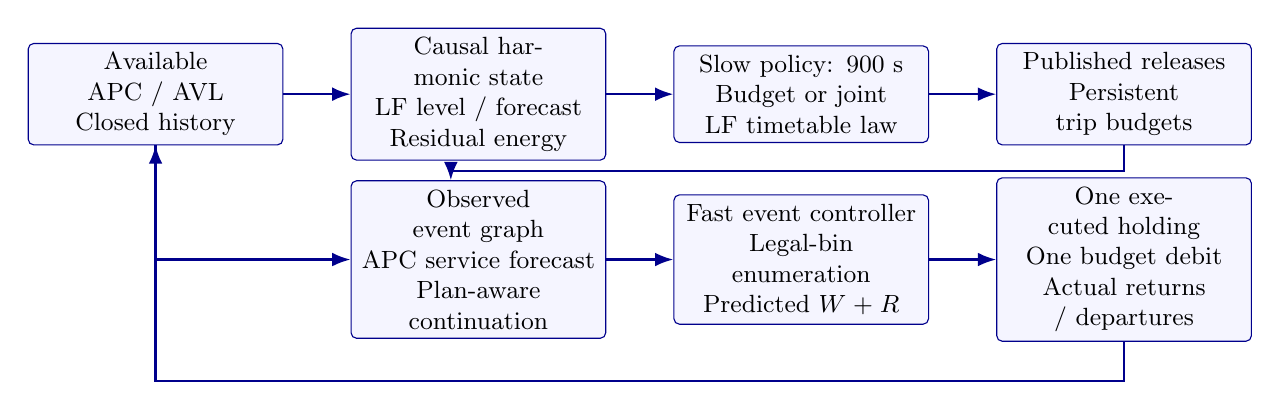
\begin{tikzpicture}[font=\small,>=Latex,
 box/.style={draw=blue!55!black,rounded corners=2pt,fill=blue!4,align=center,minimum height=1.0cm,text width=3.0cm},
 arr/.style={->,thick,blue!55!black}]
\node[box] (data) at (0,0) {Available APC / AVL\\Closed history};
\node[box] (freq) at (4.1,0) {Causal harmonic state\\LF level / forecast\\Residual energy};
\node[box] (slow) at (8.2,0) {Slow policy: 900 s\\Budget or joint\\LF timetable law};
\node[box] (ledger) at (12.3,0) {Published releases\\Persistent trip budgets};
\node[box] (graph) at (4.1,-2.1) {Observed event graph\\APC service forecast\\Plan-aware continuation};
\node[box] (fast) at (8.2,-2.1) {Fast event controller\\Legal-bin enumeration\\Predicted $W+R$};
\node[box] (physical) at (12.3,-2.1) {One executed holding\\One budget debit\\Actual returns / departures};
\draw[arr] (data)--(freq);
\draw[arr] (freq)--(slow);
\draw[arr] (slow)--(ledger);
\draw[arr] (data.south) |- (graph.west);
\draw[arr] (ledger.south) -- ++(0,-.32) -| ([xshift=-.35cm]graph.north);
\draw[arr] (graph)--(fast);
\draw[arr] (fast)--(physical);
\draw[arr] (physical.south) -- ++(0,-.5) -| (data.south);
\end{tikzpicture}
\caption{Implemented information and resource pathways. Frequency summaries inform the slow policy and timetable law. The fast layer uses APC/AVL, published plans, and remaining budgets; no direct high-frequency demand-residual branch is assumed. Physical events update the observations and resource ledger.}
\label{fig:architecture}
\end{figure*}

\subsection{Causal Frequency Summaries}
The frequency tracker forms closed-bin APC signals and maintains a causal harmonic state. For a nonnegative observed rate $x_n$, let $z_n=\log(1+x_n)$ and let $\phi_n$ contain an intercept, a temporal trend, and harmonic basis terms. A recursive least-squares update has the form
\begin{align}
 k_n&=\frac{P_{n-1}\phi_n}{\rho+\phi_n^\top P_{n-1}\phi_n},\\
 \theta_n&=\theta_{n-1}+k_n(z_n-\phi_n^\top\theta_{n-1}),\\
 P_n&=\rho^{-1}(P_{n-1}-k_n\phi_n^\top P_{n-1}).
\end{align}
The transformed fitted value supplies a nonnegative low-frequency summary $L_n$. A residual is formed against the \emph{pre-update} prediction, and its smoothed value and energy are retained. Thus the fitted low component and smoothed residual are not an exact additive reconstruction of the raw count. A future low-frequency summary is obtained by evaluating the fitted state at the future harmonic phase, without incorporating future observations.

The implemented slow state includes global low demand, its slope, a low-frequency forecast, and high-frequency energy. The timetable rule uses the global low level and forecast. Station-specific short-window arrival-rate estimates in the fast graph are obtained separately from APC clearance intervals. They have units of passengers per second and are not interchangeable with boarding-bin residuals. This separation avoids adding quantities with different sampling and exposure meanings.

\subsection{Bounded Dynamic Timetable Revision}
The slow manager begins at 7200 s and considers publication every 900 s. For each direction, a revision concerns the next mutable departure and preserves the following departure as an anchor. Write $p_1$ for the next public release, $p_2$ for the following public release, and $d_-$ for the preceding actual departure. Let $L_t$ and $F_t$ be the currently supported low-frequency level and forecast. Define
\begin{align}
 \omega_t&=\clip((p_2-t)/1800,0,1),\\
 \ell_t&=\pos{L_t},\qquad r_t=\pos{(1-\omega_t)L_t+\omega_t F_t},\\
 \tau^*&=\frac{\ell_t d_-+r_t p_2}{\ell_t+r_t}.
 \label{eq:timetable}
\end{align}
If the frequency estimate is unsupported, equal weights replace $\ell_t$ and $r_t$. The proposed release is restricted to a $\pm30$ s shift around $p_1$, then constrained by the current time, a 180 s minimum separation from the preceding published release, and a 180 s separation from the anchor. The executable value is rounded upward to the simulator's integer-second clock. Both the revised trip's target headway and the anchor's following target headway are updated.

A revision requires two mutable future departures within the publication window, sufficient completed-trip history, and a compatible vehicle-supply estimate. A trip that has already become operationally committed is not rewritten. The rule evaluates supply from available vehicles and forecast returning vehicles; it does not create an additional vehicle or reserve an unobserved return. Consequently, a proposed plan can be rejected even when its demand-weighted release is attractive. The learned policy controls permission to invoke this law, rather than directly optimizing all timetable entries.

\subsection{Persistent Holding Budgets}
For each active vehicle--trip pair $i$, the manager estimates the normal remaining command exposure $C_i$ from the number of remaining controls and the median command seconds per control in at least three completed eligible trips of the same direction. A return estimate separates the remaining non-holding running and service component, irrevocable commands, and the physical overhead of control events. It is matched to an upcoming trip within a 2700 s supply look-ahead.

Let $\widehat r_i^{\mathrm{ord}}$ be the estimated ordinary return time, and $p_{j(i)}$ the public departure of the matched trip. The estimated supply pressure and proposed remaining allowance are
\begin{align}
 P_i&=\pos{\widehat r_i^{\mathrm{ord}}+1-p_{j(i)}},\\
 \widetilde B_i&=\left\lceil\max(\rho_B C_i,C_i-P_i)\right\rceil.
 \label{eq:budget}
\end{align}
The main experiment uses $\rho_B=0.5$; the prespecified configuration study also evaluates 0.25 and 0.75 without retraining. This retention floor preserves a fraction of the estimated ordinary command exposure; a larger value permits more holding time at the same supply pressure. It is a time allowance, not a vehicle or driver fraction. Only active trips with positive pressure, positive normal exposure, and remaining control opportunities receive a new allowance. If an allowance already exists, publication takes $\min(B_i,\widetilde B_i)$ rather than replenishing it. At final submission of a command,
\begin{equation}
 B_i\leftarrow B_i-h_e,\qquad h_e\leq B_i^{\mathrm{before}}.
 \label{eq:debit}
\end{equation}
The allowance is closed when that trip returns. It persists across changes in the upper mode and across all remaining control points.

Budget accounting uses command seconds. In the simulator, a zero command still occupies one physical tick at a control point. Thus physical residence is $\max(1,h_e)$ for a submitted command, with corresponding automatic zero ticks at unrequested controls. Treating residence as identical to the budget debit would change the executed model. The return predictor estimates this overhead separately; it does not claim that subtracting one budget second always advances a return by one second.

\subsection{Fast Holding with a Common Continuation}
At a controllable event, the fast layer constructs a graph from the same current observations, published plans, and budget ledger. Its reference is the native bilateral rule projected onto the remaining allowance. If the native command is $h_e^{\mathrm{nat}}$, the projection is
\begin{equation}
 \bar h_e=\max\{h\in\mathcal H_e:h\leq h_e^{\mathrm{nat}},\ h\leq B_i\},
 \label{eq:projection}
\end{equation}
where the budget restriction is omitted for an unbudgeted trip. The rule's original legal mask is preserved. The current controller enumerates the legal members of $\{0,5,10,15,20,30,45\}$ s, using the same future native continuation and a separate copy of the ledger for each evaluation. The selected action minimizes predicted $W+R$ over candidates that satisfy the frozen relative feasibility conditions: predicted CV$^2$, relevant vehicle return times, subsequent departure times, and trip departure delays must not exceed their reference values. Coverage must be complete for the required events. The first executable command is applied; future actions remain predictions.

Published releases affect terminal events and downstream supply matching in the graph. Budget depletion changes later available commands. These dependencies mean that the two layers interact through a shared feasible set, even if the immediate passenger-cost ordering of the current holding candidates does not change. Every trial starts from the same remaining allowance, so searching more candidates does not spend physical budget. Only the executed command debits the live ledger.

If the predictive reference lacks the required support, the controller uses the budget-feasible native command. This fallback is an operational part of the method. An enumeration can be exact over the current finite library and still fail to identify the best real-world action, because the future continuation and demand estimates are approximate. We therefore distinguish search completeness from prediction accuracy and from actual transport benefit.

\subsection{Learning the Slow Publication Mode}
The upper action set is $\mathcal A=\{\mathrm{budget},\mathrm{joint}\}$. Both modes permit persistent budgets; only the joint mode permits a new timetable revision. The 180-dimensional state contains the time, fleet load, frequency summaries, accumulated arrival-headway moments, public-delay debt, the previous mode, directional supply and plan summaries, completed-trip history, and telemetry and remaining allowances for the 12 vehicles. Fixed divisors normalize these fields. The same canonical action labels are used in the actor, critic, replay, previous-action encoding, and execution.

The reward is the negative increment of~\eqref{eq:objective} over a slow interval. With $\gamma=1$ and a finite daily episode, interval increments retain their daily accounting interpretation. The final interval is closed after the service tail. A discrete maximum-entropy actor--critic uses twin critics and the target
\begin{align}
 V(s')&=\sum_{a'}\pi(a'|s')\left[\min_m\bar Q_m(s',a')-\alpha\log\pi(a'|s')\right],\\
 y&=r+(1-d)V(s').
\end{align}
where $d$ denotes termination. The actor minimizes
\begin{equation}
 L_\pi=\E_s\sum_a\pi(a|s)\left[\alpha\log\pi(a|s)-\min_m Q_m(s,a)\right].
\end{equation}
The entropy temperature is fixed at $10^{-5}$, the hidden width is 64, the learning rate is $3\times10^{-4}$, and the target update coefficient is 0.005. Replay capacity is 8192. Training behavior mixes the policy with a 0.1 uniform exploration component; evaluation uses the deterministic policy. These settings are held fixed for the action-semantics comparison.

\begin{algorithm}[t]
\caption{One interaction cycle of FreqDuet}
\label{alg:control}
\begin{algorithmic}[1]
\STATE Update histories from newly available APC/AVL events.
\IF{a new slow publication time has been reached}
\STATE Close the preceding reward interval; encode current state.
\STATE Select budget or joint using the upper policy.
\STATE Issue or tighten trip budgets using~\eqref{eq:budget}.
\IF{joint is selected and a plan revision is supported}
\STATE Publish the bounded release and its two target headways.
\ENDIF
\ENDIF
\IF{a vehicle requests a holding action}
\STATE Build the observed graph with current plans and budgets.
\STATE Project the native reference using~\eqref{eq:projection}.
\STATE Enumerate current legal candidates with separate ledgers.
\STATE Select the lowest-cost feasible action or reference fallback.
\STATE Submit one command and debit its live trip allowance once.
\ENDIF
\STATE Close the allowance when its physical trip returns.
\end{algorithmic}
\end{algorithm}

\subsection{What the Architecture Identifies}
The architecture makes two interactions explicit: slow releases alter fast resource feasibility, and fast holding consumes vehicle time that constrains later releases. It also exposes a useful distinction between \emph{permission} and \emph{dose}. Selecting joint does not guarantee that a plan will be revised; the law may reject a publication, produce the same integer-second release, or be unable to influence an already committed trip. An upper action count is therefore insufficient evidence of timetable control. We record published revisions, binding to actual departures, and changes relative to matched control paths.

Similarly, an enabled frequency feature is not evidence of beneficial frequency specialization. The verified pathway is frequency summary to slow state or plan law, then published plans and budgets to fast control. A direct high-frequency residual correction to station demand or holding is outside the evaluated main implementation. The architecture figure depicts only these implemented paths. This scope permits a reproducible method description while keeping a stronger LF/HF division-of-labor hypothesis testable.

\section{Properties of the Coordination Interface}
\label{sec:properties}
The interface admits several limited statements that help interpret the experiments. They concern the meaning of the executed commands and comparisons, rather than optimality of the learned policy.

\subsection{Cumulative Feasibility of a Trip Budget}
Suppose a trip first receives allowance $B_0\geq0$. Let $h_1,\ldots,h_m$ be its subsequently committed holding commands and let $u_1,\ldots,u_q\geq0$ be the reductions imposed by later budget publications. If each command is constrained by the currently remaining allowance and debited exactly once, then
\begin{equation}
 B_{\mathrm{rem}}=B_0-\sum_{e=1}^{m}h_e-\sum_{v=1}^{q}u_v\geq0.
 \label{eq:budget_identity}
\end{equation}
This follows by induction over the ordered sequence of command submissions and publications. A legal submission subtracts at most the current remainder. A publication replaces the remainder by the minimum of itself and a nonnegative proposal, subtracting a nonnegative reduction. Neither event increases the allowance. Consequently, total committed holding after issuance cannot exceed $B_0$, regardless of how often the upper mode changes.

The same identity holds inside an individual predictive continuation because its ledger uses the same events. It does not imply a realized return-time bound: uncertain running and service times, control-point residence, and later dispatch availability remain outside this scalar accounting identity. It also does not compare total holding with an unconstrained policy that would visit different future states. Its practical value is that prediction and execution refer to the same limited resource.

\subsection{Timetable Revision Redistributes Adjacent Targets}
Let $\tau_-$ be the preceding published release. Before a permitted revision, the two adjacent target headways are $p_1-\tau_-$ and $p_2-p_1$. After changing the next release to $\tau_1$, they become $\tau_1-\tau_-$ and $p_2-\tau_1$. Therefore,
\begin{equation}
 (\tau_1-\tau_-)+(p_2-\tau_1)=p_2-\tau_-.
 \label{eq:anchor}
\end{equation}
The law redistributes service within a fixed anchored span. It neither inserts a trip nor increases the nominal fleet. The term ``frequency-informed'' refers to temporal components of the observed signal, rather than an increase in the total scheduled service frequency. As actual releases depend on vehicle availability,~\eqref{eq:anchor} describes published targets and does not force realized headways to attain those values.

This limited intervention also explains why many budget and joint choices can be behaviorally identical. The same state may yield no mutable departure, an unsupported supply estimate, an unchanged rounded release, or a release whose effect is absorbed before dispatch. A critic trained on the mode label then learns across both effective and ineffective interventions. The relevant learning question is whether state information identifies the occasions on which a permitted revision changes passenger outcomes, not whether the actor selects joint often.

\subsection{Identical Cost Rankings Can Produce Different Actions}
Let $\widehat C(h)$ be the predicted passenger cost of a current action, and let $\mathcal F(\tau,B)$ be its feasible set under the published plan and remaining budget. The fast decision is
\begin{equation}
 h^*(\tau,B)\in\arg\min_{h\in\mathcal F(\tau,B)}\widehat C(h).
\end{equation}
Even if a plan change leaves $\widehat C(h_1)<\widehat C(h_2)$ intact, it can switch the selected action by removing $h_1$ from the feasible set. A change in the fast command is thus evidence of operational coupling without, by itself, proving that the new plan improves passenger cost. The matched capture in the experiments provides precisely this kind of observation. It is a useful mechanism test because all retained non-plan inputs can be held equal.

\subsection{Consistent Windows for Regularity Comparisons}
For $n$ included arrival headways with sum $S$ and squared sum $Q$, the population-moment convention gives
\begin{equation}
 \mathrm{CV}^2=\frac{nQ}{S^2}-1,\qquad n>0,\ S>0.
 \label{eq:cv_moments}
\end{equation}
The fast model extends an observed prefix with a predicted suffix. A physical short continuation may end before some of the suffix events occur. Comparing its CV$^2$ with a complete model rollout then changes $n$, $S$, and $Q$ together. Even the sign of an action difference can change when a single boundary event is included. Our diagnostic recomputes all three quantities on a common observation window before interpreting a sign disagreement as a prediction failure. Window alignment does not correct inaccurate event times; it makes the comparison address the same set of temporal obligations.

Together, these properties locate the method's guarantees at the interface: cumulative command feasibility, anchored plan semantics, and well-defined comparisons. Realized waiting-time improvement, vehicle readiness, and generalization remain empirical questions.

% Sources: experiments/v326_two_action_upper/{RESULTS.md,PROTOCOL.md,config.json,review01/aggregate.json}
% Sources: experiments/v325_budget_permission/{RESULTS.md,review01/aggregate.json}
% Sources: experiments/v316_upper_no_cv/learning01/{RESULTS.md,config.json}
% Sources: experiments/v331_candidate_capture/RESULTS.md
% Source: experiments/v350_live_basis_wiring/matched_launch01/review01/matched_aggregate.json
% Source: experiments/v352_budget_interface/review01/aggregate.json
% Source: experiments/v399_equal_budget_manual/review01/compare.json
% All estimates below are transcribed from existing server aggregates, not recomputed.

\section{Experimental Evaluation}
\label{sec:experiments}

The evaluation separates three questions: how learned and strong manual joint
control compare at matched budget retention, how retention changes service and
regularity, and what harmonic terms contribute under matched retraining.
Historical objective and authorization comparisons provide additional context.
The preselected default candidate and its retention of 0.5 remain unchanged.

\subsection{Experimental Design and Comparators}

The simulated corridor has 22 physical stops, including two terminals, with
21 segments of 500 m in each direction (10.5 km one way). Each bus has capacity
50. The public timetable specifies 131 trips per direction at 360-s intervals;
the two initial departures are offset by 180 s. Time zero corresponds to
06:00. The simulation advances in 1-s steps, updates road conditions every
300 s, and generates passengers in 20-s windows from the configured hourly
origin--destination table. Counts are Poisson, with arrival times sampled
uniformly within each window and revealed only when they occur. The scenario
generator perturbs hourly demand and shifts the hourly template. Link speeds
are sampled around hourly means, clipped to the supported range, and used in
the physical vehicle update. This is a stochastic simulation study; the
development demand seeds are not independent observations from an operational
deployment.

The nominal demand cutoff is the last public departure at 46,980 s. A
14,400-s service tail gives a maximum accounting horizon of 61,380 s; physical
driving can end earlier when service has finished. Passenger metrics are
restricted accumulated times over this evaluation horizon. They include
waiting for generated passengers who remain unserved, rather than conditioning
on completed journeys. Accordingly, ``journey'' below means the sum of
accounted waiting and onboard exposure per generated passenger, not an assertion
that every generated passenger has reached a destination.

All reported full-day comparisons retain the same 12-vehicle fleet, 262 scheduled
trips, demand realization within each paired day, and fast holding controller.
Passenger accounting includes the prescribed waiting and onboard tail. Waiting
and onboard time are divided by the number of passengers generated on the same
day; journey time is their sum. Vehicle-readiness delay is normalized by 262
trips, while public departure delay is reported as a daily total relative to the
unchanged public timetable. Consequently, revising an internal operating plan
cannot erase a public delay by redefining its reference. Actual headway
\(CV^2\) is reported separately from these service measures.

The four-mode learner and FreqDuet each use three initialization seeds, 314011,
314037, and 314049. Each seed receives 32 distinct training demand days, identifiers
1780001--1780032, in eight batches of four days. A batch uses its preceding
checkpoint and is followed by 192 updates, giving 1,536 updates per seed and
4,608 in total. The final checkpoint is evaluated deterministically without
updates on demand days 2077001--2077004. Seed 314011 and its eighth-batch
checkpoint were designated before evaluation as the primary candidate; the
other seeds assess sensitivity rather than provide alternative candidates for
selection. The four evaluation days had already been used during development.

The comparators isolate different parts of the coordination mechanism.
\emph{Fixed plan} retains the original upper timetable with the same fast
controller. The \emph{four-mode learner} chooses among fixed, plan, budget, and
joint permissions using the passenger-and-delay objective. The
\emph{permission-mapped learner} freezes that actor and maps fixed to budget and
plan to joint, retaining its weights, prediction inputs, and fast controller.
This intervention provides budget authorization at every upper decision but
does not retrain the critic under the changed action semantics.
\emph{Manual joint} always authorizes the same low-frequency plan rule and
holding-budget mechanism. It is therefore a strong coordinated comparator,
not an uncontrolled schedule. FreqDuet instead learns directly between the two
executable budget and joint actions, with actor, critic, replay labels, previous
action encoding, and execution sharing the same semantics (archived as V326,
V316, and V325 for FreqDuet, the four-mode learner, and the permission-mapped
learner, respectively). For seed-sensitivity comparisons, the four-mode and
permission-mapped references both use their frozen seed-314011 policies; manual
joint is also shared across the three FreqDuet seeds.

The optimization objective is given in~\eqref{eq:objective}.

For the main comparison, both learned and manual joint control use retention
$\rho_B=0.5$ and $0.25$. The latter manual arm is evaluated on the same four
days with no learning; the learned arms and the default manual arm are reused
from the existing evaluations. Equal retention means the same lower bound in
the allowance formula, not equal realized allowance, holding, or state
trajectory. The additional manual paths each complete all 262 trips, preserve
the 12-vehicle pool, and match 5,200 common random events per day. The original
default manual path is reproduced before applying the tighter setting.

Differences are always method minus the named comparator, so negative values
denote reductions. The archived summaries use equal day weights and all $4^4=256$ paired
resamples with replacement from the four days. We retain their descriptive 95\% intervals
and report each learning seed separately. Twelve evaluation runs represent
three policies on four demand days, not twelve independent demand days.

\subsection{Main Comparison at Matched Budget Retention}
\label{sec:equal_budget}

Table~\ref{tab:equal_budget} reports the four controller--retention combinations.
At retention 0.25, the learned policy reduces mean journey time by only
0.094~s/passenger relative to strong manual joint control. The corresponding
waiting, journey, readiness, and actual $CV^2$ intervals all span zero.
Journey differences by day are $+0.883$, $+0.163$, $+0.336$, and $-1.758$
s/passenger; waiting also improves only on the fourth day. At default retention
0.5, the mean journey difference is larger at $-1.925$~s/passenger, but its
interval also spans zero. The main outcome is therefore a matched description
of operational performance, not an established learning advantage.

\begin{table*}[t]
\centering
\caption{Matched-retention main comparison on four reused development days.
The learned policy is the preselected K4 candidate; manual joint is a strong
coordinated controller. Retention is an allowance floor, not realized holding.
Intervals in panel (b) are descriptive paired 95\% intervals.}
\label{tab:equal_budget}
\small
\textbf{(a) Absolute means}\par\smallskip
\setlength{\tabcolsep}{8pt}
\begin{tabular}{lrrrrr}
\toprule
Upper policy & $\rho_B$ & Waiting (s/passenger) & Journey (s/passenger) & Readiness (s/trip) & Actual $CV^2$ \\
\midrule
Manual joint & 0.50 & 308.775 & 998.705 & 65.450 & 0.08083 \\
Learned K4 (default) & 0.50 & 307.752 & 996.780 & 64.725 & 0.07802 \\
Manual joint & 0.25 & 307.372 & 995.285 & 62.732 & 0.08273 \\
Learned K4 & 0.25 & 307.300 & 995.191 & 62.179 & 0.08220 \\
\bottomrule
\end{tabular}
\par\medskip
\textbf{(b) Learned K4 minus manual joint at the same retention}\par\smallskip
\begin{tabular}{lrr}
\toprule
Metric & $\rho_B=0.50$ & $\rho_B=0.25$ \\
\midrule
Waiting (s/passenger) & $-1.023\;[-3.396,0.668]$ & $-0.072\;[-1.307,0.955]$ \\
Journey (s/passenger) & $-1.925\;[-5.935,0.762]$ & $-0.094\;[-1.234,0.703]$ \\
Readiness (s/trip) & $-0.725\;[-3.295,0.885]$ & $-0.552\;[-1.552,0.447]$ \\
Actual $CV^2$ & $-0.002816\;[-0.007316,0.000185]$ & $-0.000532\;[-0.001479,0.000620]$ \\
\bottomrule
\end{tabular}
\end{table*}


These small aggregate differences do not arise from identical execution. At
retention 0.25, the controllers differ in 43 trips' published release times,
245 trips' actual departures, and 3,989 matched holding commands across the
four days. These are records from different closed-loop trajectories; they
cannot identify the passenger effect of any individual command.

The matched comparison also clarifies the earlier cross-budget contrast.
Learned control at 0.25 versus manual joint at 0.5 reduces journey time by
3.514~s/passenger. Along the comparison sequence that first tightens the
manual budget and then changes upper policy at retention 0.25, this difference
is $-3.420-0.094=-3.514$~s/passenger. The waiting contrast similarly decomposes
as $-1.403-0.072=-1.475$~s/passenger. These are accounting identities along a
stated sequence, not a unique allocation of interacting causal effects.
The journey difference-in-differences is $+1.831$~s/passenger
$[-2.039,6.681]$; there is no resolved advantage in how the learned policy
responds to budget tightening. Section~\ref{sec:budget_settings} reports the
within-policy configuration effects.

\subsection{Historical Objective and Authorization Comparisons}

The historical comparisons evaluate the default preselected candidate
against earlier learners and manual joint, all at retention 0.5.
Relative to the four-mode learner, journey
time decreases by 7.448~s/passenger, vehicle-readiness delay by
12.221~s/trip, and public departure delay by 3,162.5~s/day. All four days improve
on these three measures, and their descriptive intervals remain below zero.
The largest passenger component is onboard time, reduced by
5.873~s/passenger. Holding decreases by 14.704~s/trip. The waiting reduction is
smaller and varies across days, indicating that the clearest recovered benefit
is reduced onboard burden and improved vehicle circulation.

The comparison with manual joint is materially closer. FreqDuet reduces mean
waiting by 1.023~s/passenger and journey time by 1.925~s/passenger, with lower
mean readiness and public delay. However, the corresponding intervals cross
zero. Waiting increases by 0.315 and 1.022~s/passenger on the third and fourth
days; journey time increases by 1.308~s/passenger on the fourth day. The
aggregate result therefore identifies a competitive candidate with favorable
means on this panel, rather than a demonstrated uniform improvement over
manual coordination. The comparator is retained in the main table because the
larger improvement over the four-mode learner alone would overstate the
remaining benefit attributable to learning.

Against the permission-mapped learner, retraining adds only
0.365~s/passenger of mean journey reduction and 0.271~s/passenger of waiting
reduction. Readiness and public delay increase slightly. This small difference
shows that most of the full-day recovery was already present after enabling
budget authorization. Correcting the action representation makes learning
consistent with execution, but does not itself establish an additional traffic
benefit.

\subsection{Objective and Authorization Ablations}

The objective ablation retains the four-mode architecture and training budget
while removing the upper regularity term from
\(J_1=J_0+CV^2/0.05\). For the preselected seed, the resulting four-mode learner
reduces journey time by 7.258~s/passenger relative to its regularity-penalized
counterpart. Relative to fixed plan, its journey reduction is
7.047~s/passenger [\(-11.169,-2.360\)], readiness decreases by
23.120~s/trip, and public delay decreases by 6,007~s/day. The two other seeds
also reduce journey time against fixed plan, by 12.296 and 9.987~s/passenger.
The action records show that budget and joint permissions become active after
the objective change; the regularity-penalized learners had selected neither
mode in their final evaluations.

This recovery includes a real regularity tradeoff. For the preselected seed,
actual \(CV^2\) increases by 0.01894 [0.01334,0.02454] against fixed plan.
Although \(J_0\) decreases by 0.10374, evaluating the same trajectories with
\(J_1\) increases cost by 0.27498. Thus the objective change exposes a useful
passenger--circulation tradeoff; it does not make the old composite criterion
pass. The four-mode learner also remains 5.523~s/passenger worse than manual
joint in journey time, on average, with all four days worse.

The authorization ablation then freezes this actor and changes only its
permission mapping. Relative to the unmapped four-mode learner, it reduces
journey time by 7.083~s/passenger [\(-15.617,-1.896\)], readiness by
12.658~s/trip [\(-22.407,-4.824\)], and public delay by
3,324.5~s/day [\(-5883.8,-1275.5\)]. Its onboard reduction is
5.779~s/passenger, while the waiting reduction of 1.304~s/passenger has an
interval spanning zero. Persistent-budget accounting confirms that existing
allowances are consumed rather than replenished at repeated decision times.
These results support authorization as an important source of the recovered
benefit. They do not isolate every indirect effect, because changed holding
also changes subsequent vehicle supply and plan opportunities.

\subsection{Learning Sensitivity and Executed Plan Authority}

Table~\ref{tab:seed_results} reports all final learning seeds. Each has lower
mean waiting and journey time than manual joint, but only the preselected seed
improves mean waiting against the permission-mapped learner. The other seeds
increase waiting by 0.341 and 0.270~s/passenger against that comparator. The
budget/joint action counts also differ substantially, despite identical action
semantics and training budgets. This variation limits the interpretation of the
small incremental gain from retraining.

\begin{table}[t]
\centering
\caption{Seed sensitivity. Passenger differences are in s/passenger. MJ denotes
manual joint; PM denotes the permission-mapped learner.}
\label{tab:seed_results}
\setlength{\tabcolsep}{3pt}
\footnotesize
\begin{tabular}{lrrrr}
\toprule
Seed & $\Delta W$/MJ & $\Delta(W+R)$/MJ & $\Delta W$/PM & Budget/joint \\
\midrule
314011 & $-1.023$ & $-1.925$ & $-0.271$ & 70/118 \\
314037 & $-0.411$ & $-0.942$ & $0.341$ & 174/14 \\
314049 & $-0.482$ & $-0.822$ & $0.270$ & 106/82 \\
\bottomrule
\end{tabular}
\end{table}

The upper controller is operationally active. Under the archived criterion
requiring a matched publication, bound dispatch, and at least a 5-s actual
departure difference, the three seeds have material plan effects on four, two,
and four demand days. The preselected candidate affects seven, five, six, and
one trips across the four days. Its actor disagrees with its online twin-min
critic ranking on 51 of 188 decisions; the individual critics disagree on
38. These diagnostics distinguish valid execution from unresolved value and
policy disagreement. A critic preference is not a measured counterfactual
traffic outcome, so these counts cannot be converted into lost passenger
seconds or used to justify replacing the evaluated actor.

\subsection{Matched Harmonic-Basis Ablation}
\label{sec:harmonic_ablation}

We retain the evaluated $K=4$ harmonic representation and retrain a $K=0$
comparison from initialization with identical seeds, training days, update
counts, reward, fast controller, and action semantics. Both the actor input and
timetable law consume the same causal summary object. A frozen complete day verifies $K=4$ operational reproduction before this
ablation. The $K=0$ arm retains the intercept, trend, online adaptation, and
innovation statistics; removing four sine--cosine pairs reduces estimator
capacity from ten to two coefficients. Thus this is a matched harmonic-basis
ablation, not removal of every temporal summary.

\begin{table}[t]
\centering
\caption{Matched retraining ablation: $K4-K0$ for the preselected candidate.
Negative differences favor retaining harmonics.}
\label{tab:harmonic}
\setlength{\tabcolsep}{4pt}
\footnotesize
\begin{tabular}{lr}
\toprule
Metric & Mean [descriptive 95\% interval] \\
\midrule
Waiting (s/passenger) & $-0.404\;[-1.352,0.316]$ \\
Onboard (s/passenger) & $-0.657\;[-0.951,-0.387]$ \\
Journey (s/passenger) & $-1.061\;[-1.889,-0.233]$ \\
Readiness (s/trip) & $-0.441\;[-0.955,0.049]$ \\
Public delay (s/day) & $-93.75\;[-228.50,21.00]$ \\
$J_0$ & $-0.00713\;[-0.01249,-0.00178]$ \\
Actual $CV^2$ & $-0.000824\;[-0.002377,0.000730]$ \\
\bottomrule
\end{tabular}
\end{table}

The preselected $K4$ candidate reduces journey time on all four days
(Table~\ref{tab:harmonic}). Mean journey differences for seeds 314011, 314037,
and 314049 are $-1.061$, $-0.286$, and $-1.174$ s/passenger, respectively;
9 of 12 seed--day comparisons favor $K4$. Onboard time improves in 10 of 12
comparisons, whereas waiting improves in only six. The result supports a
modest journey benefit from retaining harmonic structure under this training
recipe. It does not establish a stable waiting benefit. Because the
intervention changes both representation capacity and the summary supplied to
the actor and plan law, their individual contributions remain coupled.
The main candidate and historical comparison rules are unchanged.

\subsection{Prespecified Budget Configuration}
\label{sec:budget_settings}

We evaluate $\rho_B\in\{0.25,0.5,0.75\}$ in~\eqref{eq:budget} using the
frozen preselected $K4$ policy. The default remains 0.5. Before evaluating the
two other settings on the same four days, one default full day reproduces all
compared actions, event times, policy states, rewards, probabilities, and
service outcomes exactly. All nine paths finish without retraining or retries;
physical, budget, action, reward, and paired random-event accounting pass.
The settings were declared in advance, and no setting replaces the main policy.

\begin{table}[t]
\centering
\caption{Prespecified budget settings relative to default $\rho_B=0.5$.
Four-day means; negative costs improve. The default contrast is zero.}
\label{tab:budget_settings}
\setlength{\tabcolsep}{6pt}
\footnotesize
\begin{tabular}{lrr}
\toprule
Metric & $\rho_B=0.25$ & $\rho_B=0.75$ \\
\midrule
Waiting (s/passenger) & $-0.452$ & $+2.015$ \\
Onboard (s/passenger) & $-1.137$ & $+2.916$ \\
Journey (s/passenger) & $-1.589$ & $+4.931$ \\
Readiness (s/trip) & $-2.546$ & $+4.401$ \\
Public delay (s/day) & $-644.75$ & $+1153.25$ \\
Holding (s/trip) & $-0.969$ & $+5.940$ \\
Actual $CV^2$ & $+0.004177$ & $+0.000196$ \\
\bottomrule
\end{tabular}
\end{table}

At 0.25, journey and readiness improve on all four days, with descriptive
95\% intervals $[-2.641,-0.541]$ s/passenger and $[-2.985,-2.168]$ s/trip.
Waiting improves on only two days; its interval is $[-1.197,0.293]$
s/passenger. Actual $CV^2$ increases on every day, with interval
$[0.000919,0.008926]$. At 0.75, journey and readiness worsen on every day,
and the waiting, journey, readiness, and public-delay intervals are above zero.
Table~\ref{tab:budget_settings} thus identifies a service--regularity tradeoff,
not a uniformly superior setting.

The tighter setting changes 4,662 matched holding actions, 30 published
releases, and 345 actual departures across the panel. Joint permissions
increase from 118 to 122 despite frozen weights: changed budgets alter later
states and hence policy decisions. Executed holding falls by 253.75 s/day;
reductions within budgeted periods are partly offset elsewhere on the changed
trajectories. These records establish a physical effect beyond changing a
logged allowance.

Against manual joint at its original retention 0.5, retention 0.25 reduces
waiting by 1.475 s/passenger $[-3.419,-0.206]$, journey by 3.514 s/passenger
$[-7.095,-0.760]$, and readiness by 3.271 s/trip $[-5.898,-1.635]$.
Waiting improves on three days and increases by 0.013 s/passenger on the fourth;
journey and readiness improve on all four. This comparison changes both
budget configuration and upper control, so it does not isolate a learning
increment at matched retention. Conversely, retention 0.75 improves $CV^2$
against manual joint on every day while worsening journey and readiness.

\subsection{Direct Coupling Between Timetable and Holding}

A paired replay provides a concrete mechanism example beyond aggregate plan
activity. At one recorded query, the effective vehicle, queue, forecast,
history, and holding-budget inputs are identical across two branches. Only the
published plan differs: one trip's release and target move by $+1$~s, and
another target moves by $-1$~s. The native reference action is 30~s, the remaining
budget is 66~s, and the same seven action bins are available.

\begin{table}[t]
\centering
\caption{Same-state timetable-to-holding interaction. Costs are predicted
passenger-seconds; a positive difference favors 20~s over 15~s.}
\label{tab:coupling}
\setlength{\tabcolsep}{4pt}
\footnotesize
\begin{tabularx}{\columnwidth}{lrrX}
\toprule
Plan branch & $C(15)-C(20)$ & Selected & Rejected alternative \\
\midrule
Budget & $142.345$ & 20~s & 15~s: 2-s plan-relative delay violation \\
Joint & $204.892$ & 15~s & 20~s: up to 1-s plan-relative delay violation \\
\bottomrule
\end{tabularx}
\end{table}

Both branches rank 20~s ahead of 15~s by passenger cost, but their plan-relative
feasible sets differ (Table~\ref{tab:coupling}). The selected action changes
from 20 to 15~s because the published plan changes which downstream departure
constraints bind. This establishes an implemented information path from the
slow plan to fast holding, rather than two disconnected controllers. It is a
local mechanism result, not a full-day synergy estimate. At another captured
query, vehicle and demand inputs have already diverged, so its changed action
cannot be attributed to the plan alone.

The same replay also illustrates the objective's meaning. The selected joint
action, relative to its 30-s reference, predicts 3,623.636 additional
person-seconds of waiting and 3,660.720 fewer onboard person-seconds, a net
37.083-person-second reduction. Minimizing their sum can therefore select an
action that increases waiting. Separating these components is essential when
interpreting a journey-time improvement.

\section{Closed-Loop Diagnostics}
\label{sec:diagnostics}

Matched continuations distinguish state prediction from prediction of a
control intervention. From one recorded state, 20 versus 30 s of holding
reduces waiting plus onboard exposure by 125 person-s under native
continuation and by 70 person-s under rolling control over the same 582-s
window. Actual cumulative CV$^2$ also decreases in both cases. Total holding
is unchanged within each pair: its location and passenger exposure change.
Reoptimization therefore attenuates this local benefit without reversing it.

Two diagnostics explain why point-forecast improvements need not improve
control. First, a predicted downstream arrival lay beyond the physical
comparison window; removing that event changed the predicted CV$^2$ difference
from approximately $+0.936\times10^{-6}$ to $-0.201\times10^{-6}$. A
cross-window sign disagreement could not establish a wrong action ranking.
Second, improved motion predictions reduced six continuous holding-target
errors below 0.562 s, yet some predictions remained across discrete-action
boundaries. For example, a predicted target of 7.9019 s and actual value of
7.3404 s straddle the 7.5-s boundary. Relevant validation must include the
projected response to an intervention and its actual continuation, not only
absolute timing error.

\section{Discussion and Evidence Boundaries}
\label{sec:discussion}

\subsection{Observation and Configuration Semantics}

A selected queue forecast of 7.0694 passengers versus a retrospective count
of one motivated an audit rather than a fitted correction. Across 441 queries
from 73 other APC intervals, interval-weighted mean error was $-0.326$
passengers and became $-1.570$ for gaps of at least 360 s. No additional eligible
target-stop observation supplied the missing arrivals, so a uniform downward
correction was unsupported. The point-correction branch was stopped.

The budget experiment gives operational meaning to configuration. The
retention floor $\rho_B$ limits the use of vehicle time while preserving
explicit timetable obligations. Its monotonic effect on a same-state
allowance does not ensure a monotonic full-day outcome. The prespecified
settings demonstrate actual service and circulation consequences, including
the regularity cost of tighter retention. They provide a concrete interface
for examining dispatch preferences. Human usability has not been measured.

\subsection{Limitations and Scope of the Claim}
\label{sec:limitations}

The learned controller's advantage over strong manual joint remains unresolved
at both matched retention settings. At retention 0.25, waiting and journey
improve only on the fourth day; intervals spanning zero establish neither
equivalence nor noninferiority. The older cross-budget contrast combines
configuration and upper-policy changes. The matched harmonic ablation supports
a modest journey increment at default retention while changing estimator
capacity and both actor and plan-law inputs. A direct high-frequency fast-control
pathway and complete LF/HF specialization remain unestablished. The fixed-fleet
implementation does not allocate vehicles or drivers by frequency band.

All full-day findings concern reused development days; independent confirmation
remains necessary. The additional manual-budget comparison uses one frozen
learning seed, whereas the default harmonic comparison reports three seeds;
the two studies do not constitute a crossed three-seed budget experiment.
The local continuation observes only seven of 24 resource endpoints and cannot
establish an all-day guarantee.

An enabled observation-vector field described as a queue estimate reads the
simulator's waiting population. It is ineligible as an additional APC
observation. The examined fast native rule does not consume that component;
future learned fast policies require an explicit observation-use audit.

A complete layer comparison should separate fixed versus dynamic timetable
control from reference versus adaptive holding under matched budgets and
observation access. A separately configured and trained TransitDuet reference
is also needed; no manual mode here is relabeled as TransitDuet. Representation-
capacity controls and independent demand days would strengthen attribution
and generalization. The current evidence supports executable coordination,
a modest harmonic increment, and measurable budget-setting tradeoffs.


\section{Conclusion}
This study develops and evaluates a coordination interface between a slow, frequency-informed timetable policy and fast holding control. Its distinguishing operational element is a persistent trip budget that is shared by prediction, action selection, and physical execution. The controller revises executable terminal releases and preserves the resulting obligations during downstream holding decisions. A matched input comparison directly demonstrates this plan-to-action coupling.

The main comparison matches both controllers' budget retention. At retention 0.25, the learned policy differs from strong manual joint control by only $-0.094$ s/passenger in mean journey time, with an interval spanning zero. The previously larger cross-budget difference largely reflects budget configuration along the stated comparison sequence. Matched retraining answers a different question: retaining harmonic terms reduces the preselected candidate's journey time by 1.061 s/passenger, with the same mean direction across all three seeds. Most of that increment is onboard time.

The resulting interface connects planning and control timescales through explicit timetable commitments and persistent command-time allowances. Tighter retention improves journey time and circulation while reducing regularity; looser retention increases passenger and vehicle delay on the evaluated panel. This is an operationally interpretable configuration effect, not a uniformly superior setting. The default candidate remains unchanged. The present evidence supports executable coordination, a modest harmonic increment, and configurable time-budget effects. It does not establish a stable learning advantage over strong manual joint control. A complete two-layer comparison, independent demand days, and expert-use evaluation remain future work.

\bibliographystyle{IEEEtran}
\bibliography{references}
\end{document}
